\documentclass[a4paper]{scrartcl}
\usepackage{tgheros}
\usepackage[T1]{fontenc}
\usepackage[all]{nowidow}

\usepackage[sorting=none]{biblatex}
\addbibresource{references.bib}

\usepackage{graphicx}
\graphicspath{{./figure}}
% \usepackage{xspace}
\usepackage{csquotes}
\usepackage{hyperref}
\usepackage[disable]{todonotes}
\usepackage{amsmath}
\usepackage{siunitx}
\usepackage{amssymb}

\newcommand{\figref}[1]{fig.\,\ref{#1}}


\begin{document}

\begin{titlepage}
\begin{center}
\vspace*{1cm}

\LARGE
  \textbf{Measurement of Voltage Noise\\in an Operational Amplifier}

\vspace{.2cm}

\normalsize
  Physical Measuring Techniques FK7063

\vspace{.5cm}
{Michael Vogt}

May 2026
\end{center}

\vspace{1cm}



\section*{Introduction}
Noise can occur in operational amplifiers (op amps) due to various effects of their internal components.
This noise is generally dependent on the frequency of operation.
The goal of this experiment is to measure the voltage spot noise density of a Burr-Brown OPA37 op amp
which corresponds to the amount of noise present at a specific frequency.

\end{titlepage}



\section{Setup}
The op amp is set up in a non-inverting amplifier circuit, see \figref{fig:opa-circuit}.
\begin{figure}[h]
  \centering
  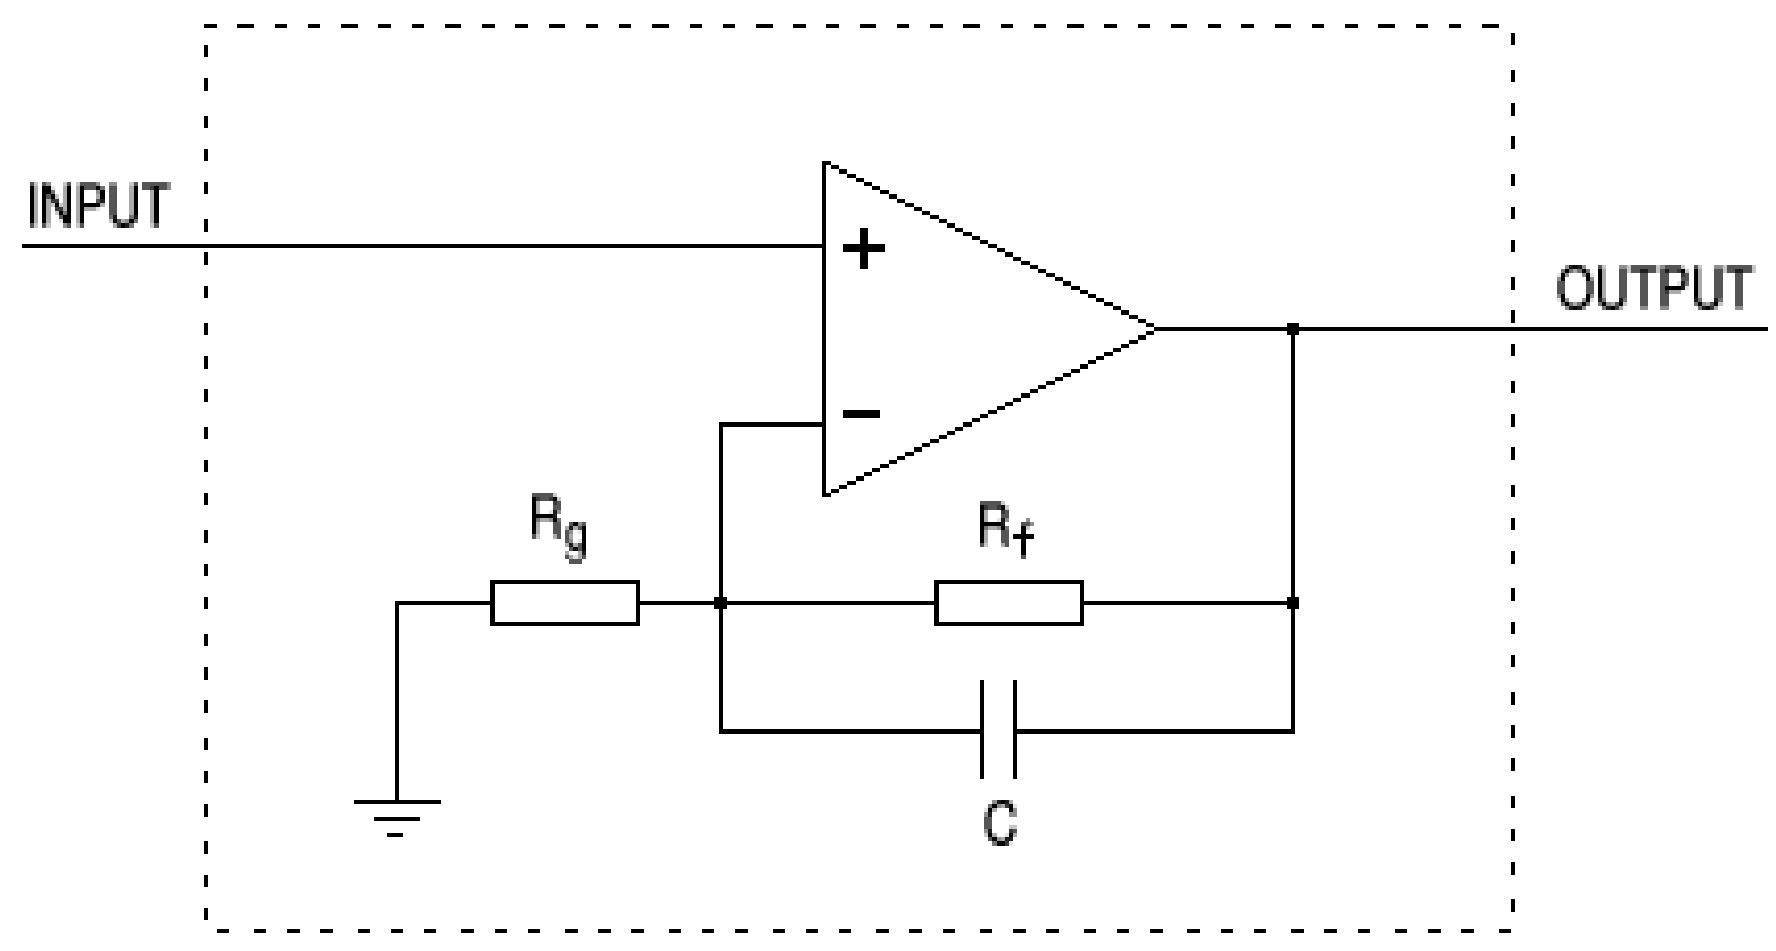
\includegraphics[width=.5\textwidth]{opa-circuit}
  \caption{non-inverting amplifier circuit. $R_f = \SI{101}{\kohm}, R_g = \SI{101}{\ohm}$ \cite{manual}}
  \label{fig:opa-circuit}
\end{figure}
The expected gain is $G=\frac{U_\text{in}}{U_\text{out}} = 1+\frac{R_f}{R_g}=1001$.
The capacitor in parallel to $R_f$ effectively lowers the resistance and therefore the gain for high frequencies,
acting as a low pass filter.
This prevents aliasing effects due to sampling of high frequencies \cite{manual}.

The input of the circuit is fed by a signal generator and the output is measured using an oscilloscope.



\section{Experiment}
First, the gain of the circuit is measured by measuring both the
input signal from the signal generator and the amplified output on the oscilloscope.

\begin{figure}[h]
  \centering
  \begin{minipage}{.5\textwidth}
    \centering
    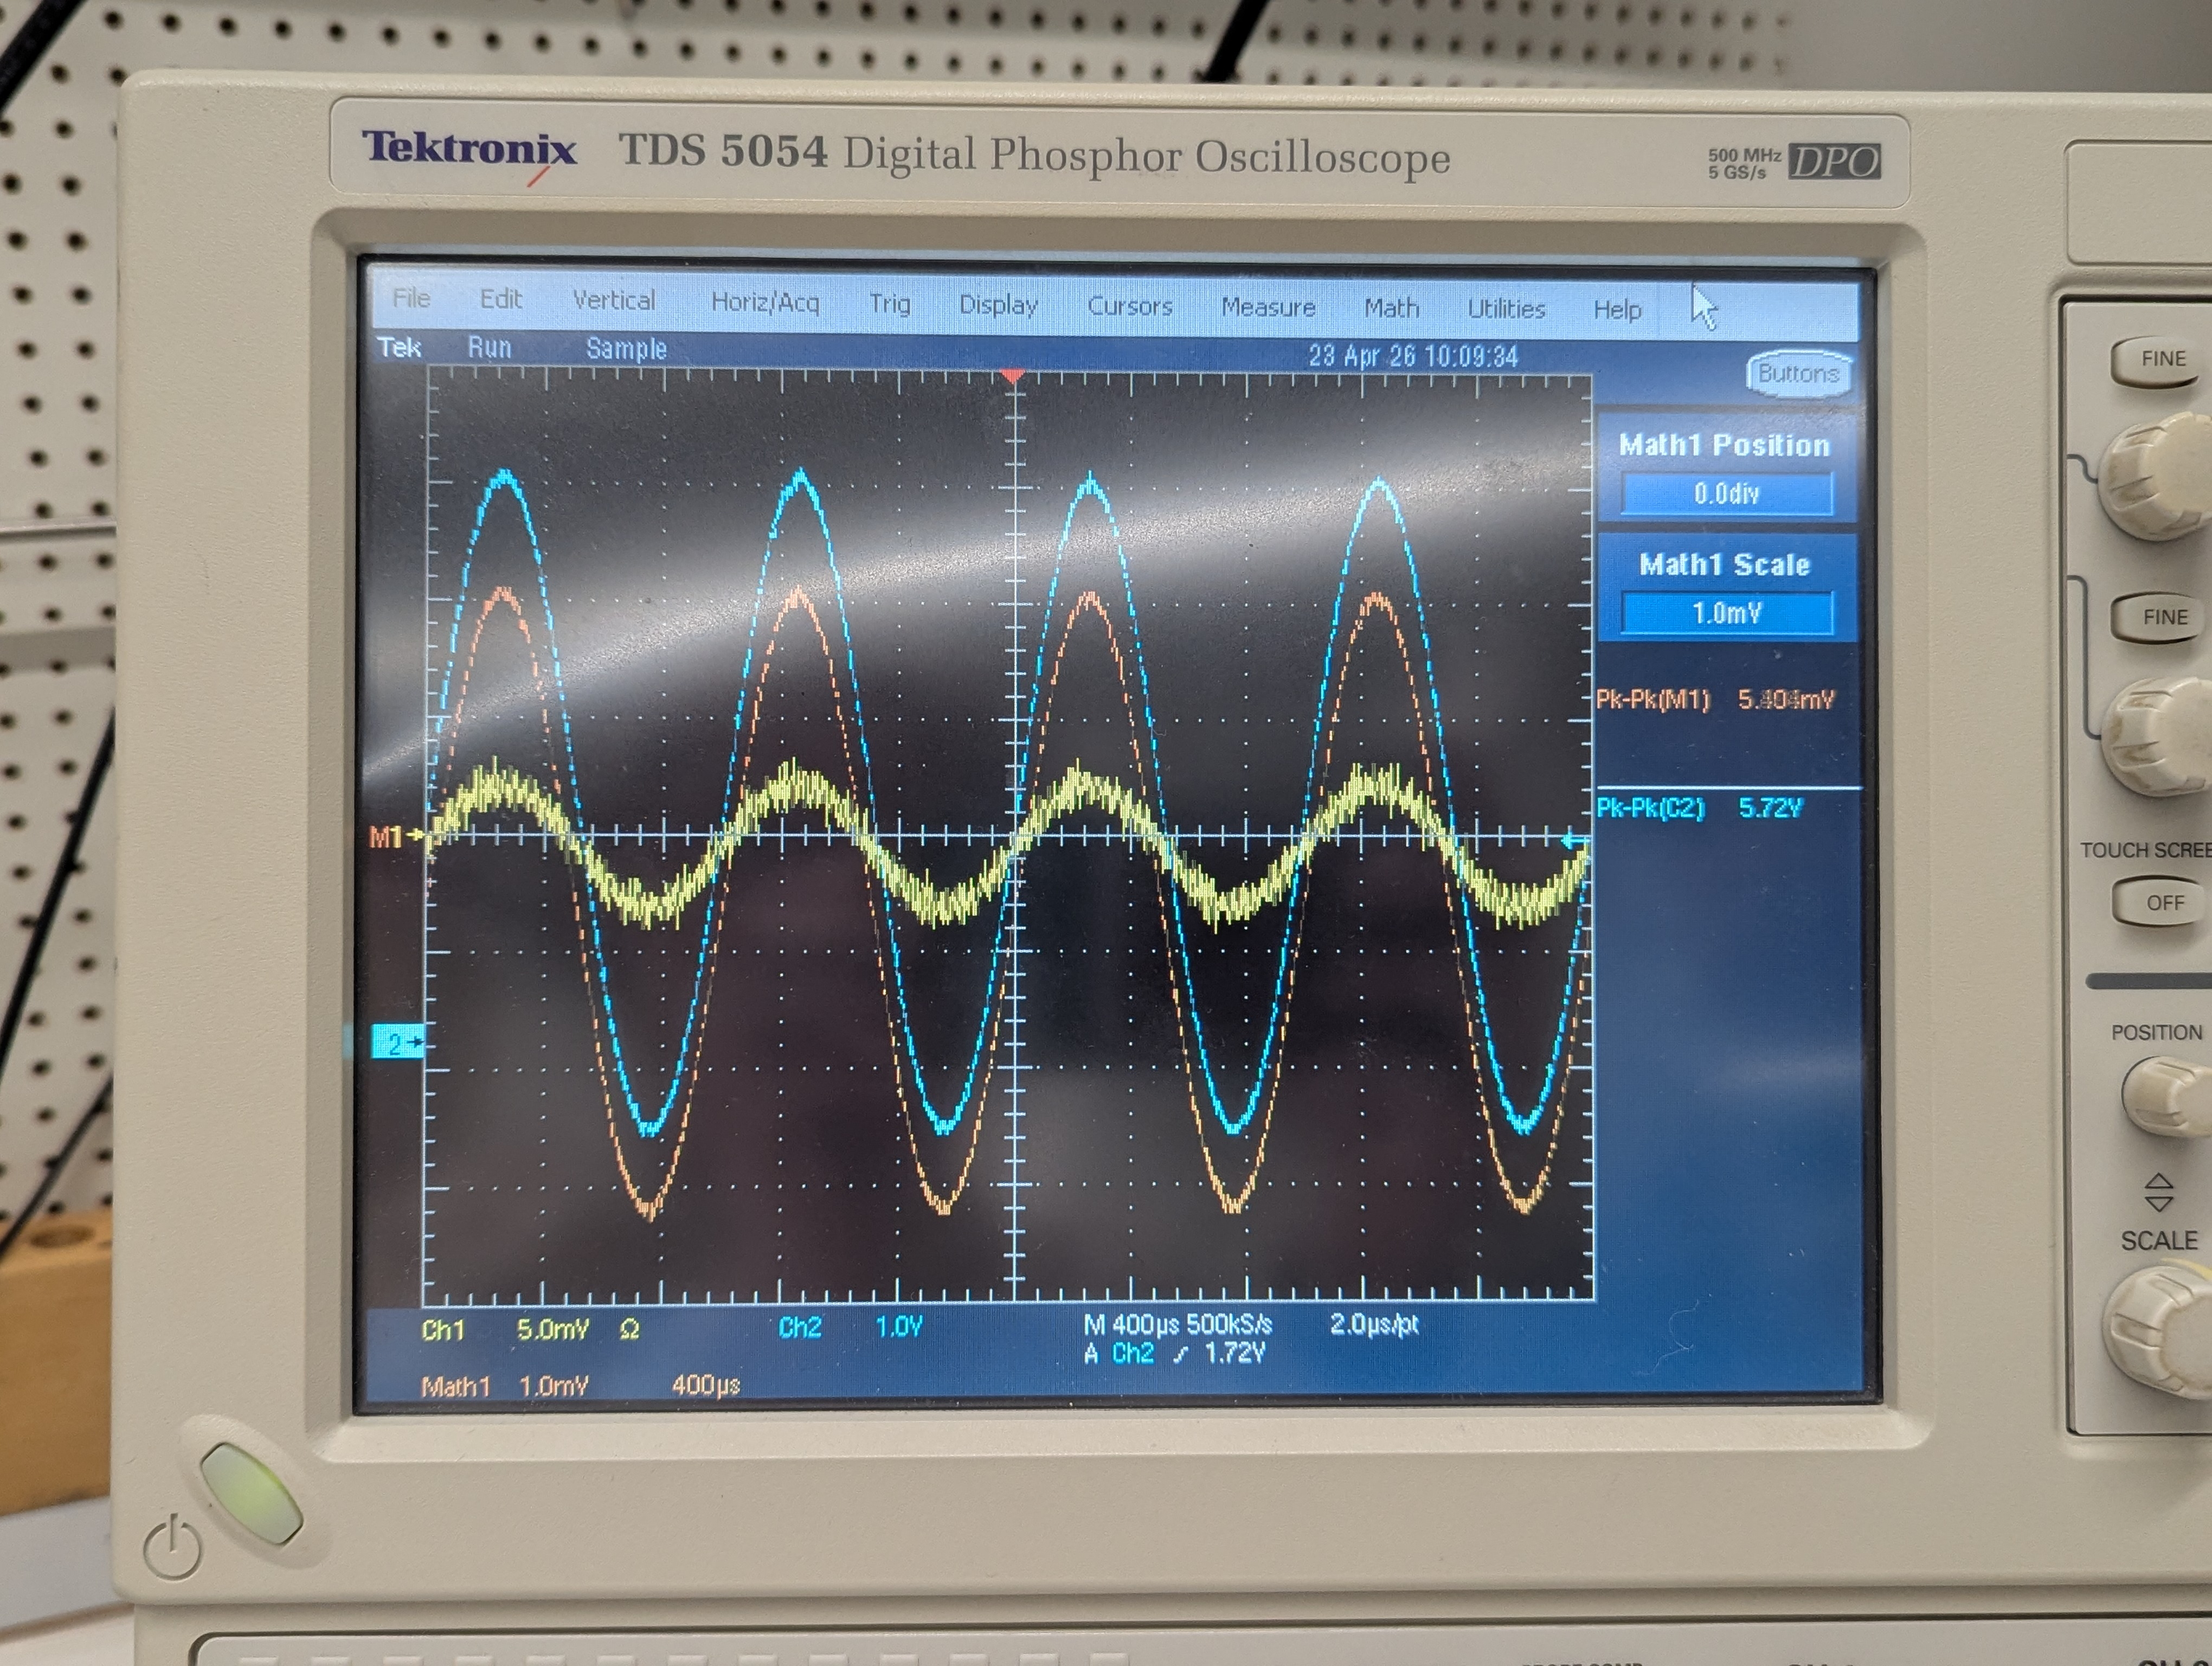
\includegraphics[width=\textwidth]{gain1.jpg}
  \end{minipage}%
  \begin{minipage}{.5\textwidth}
    \centering
    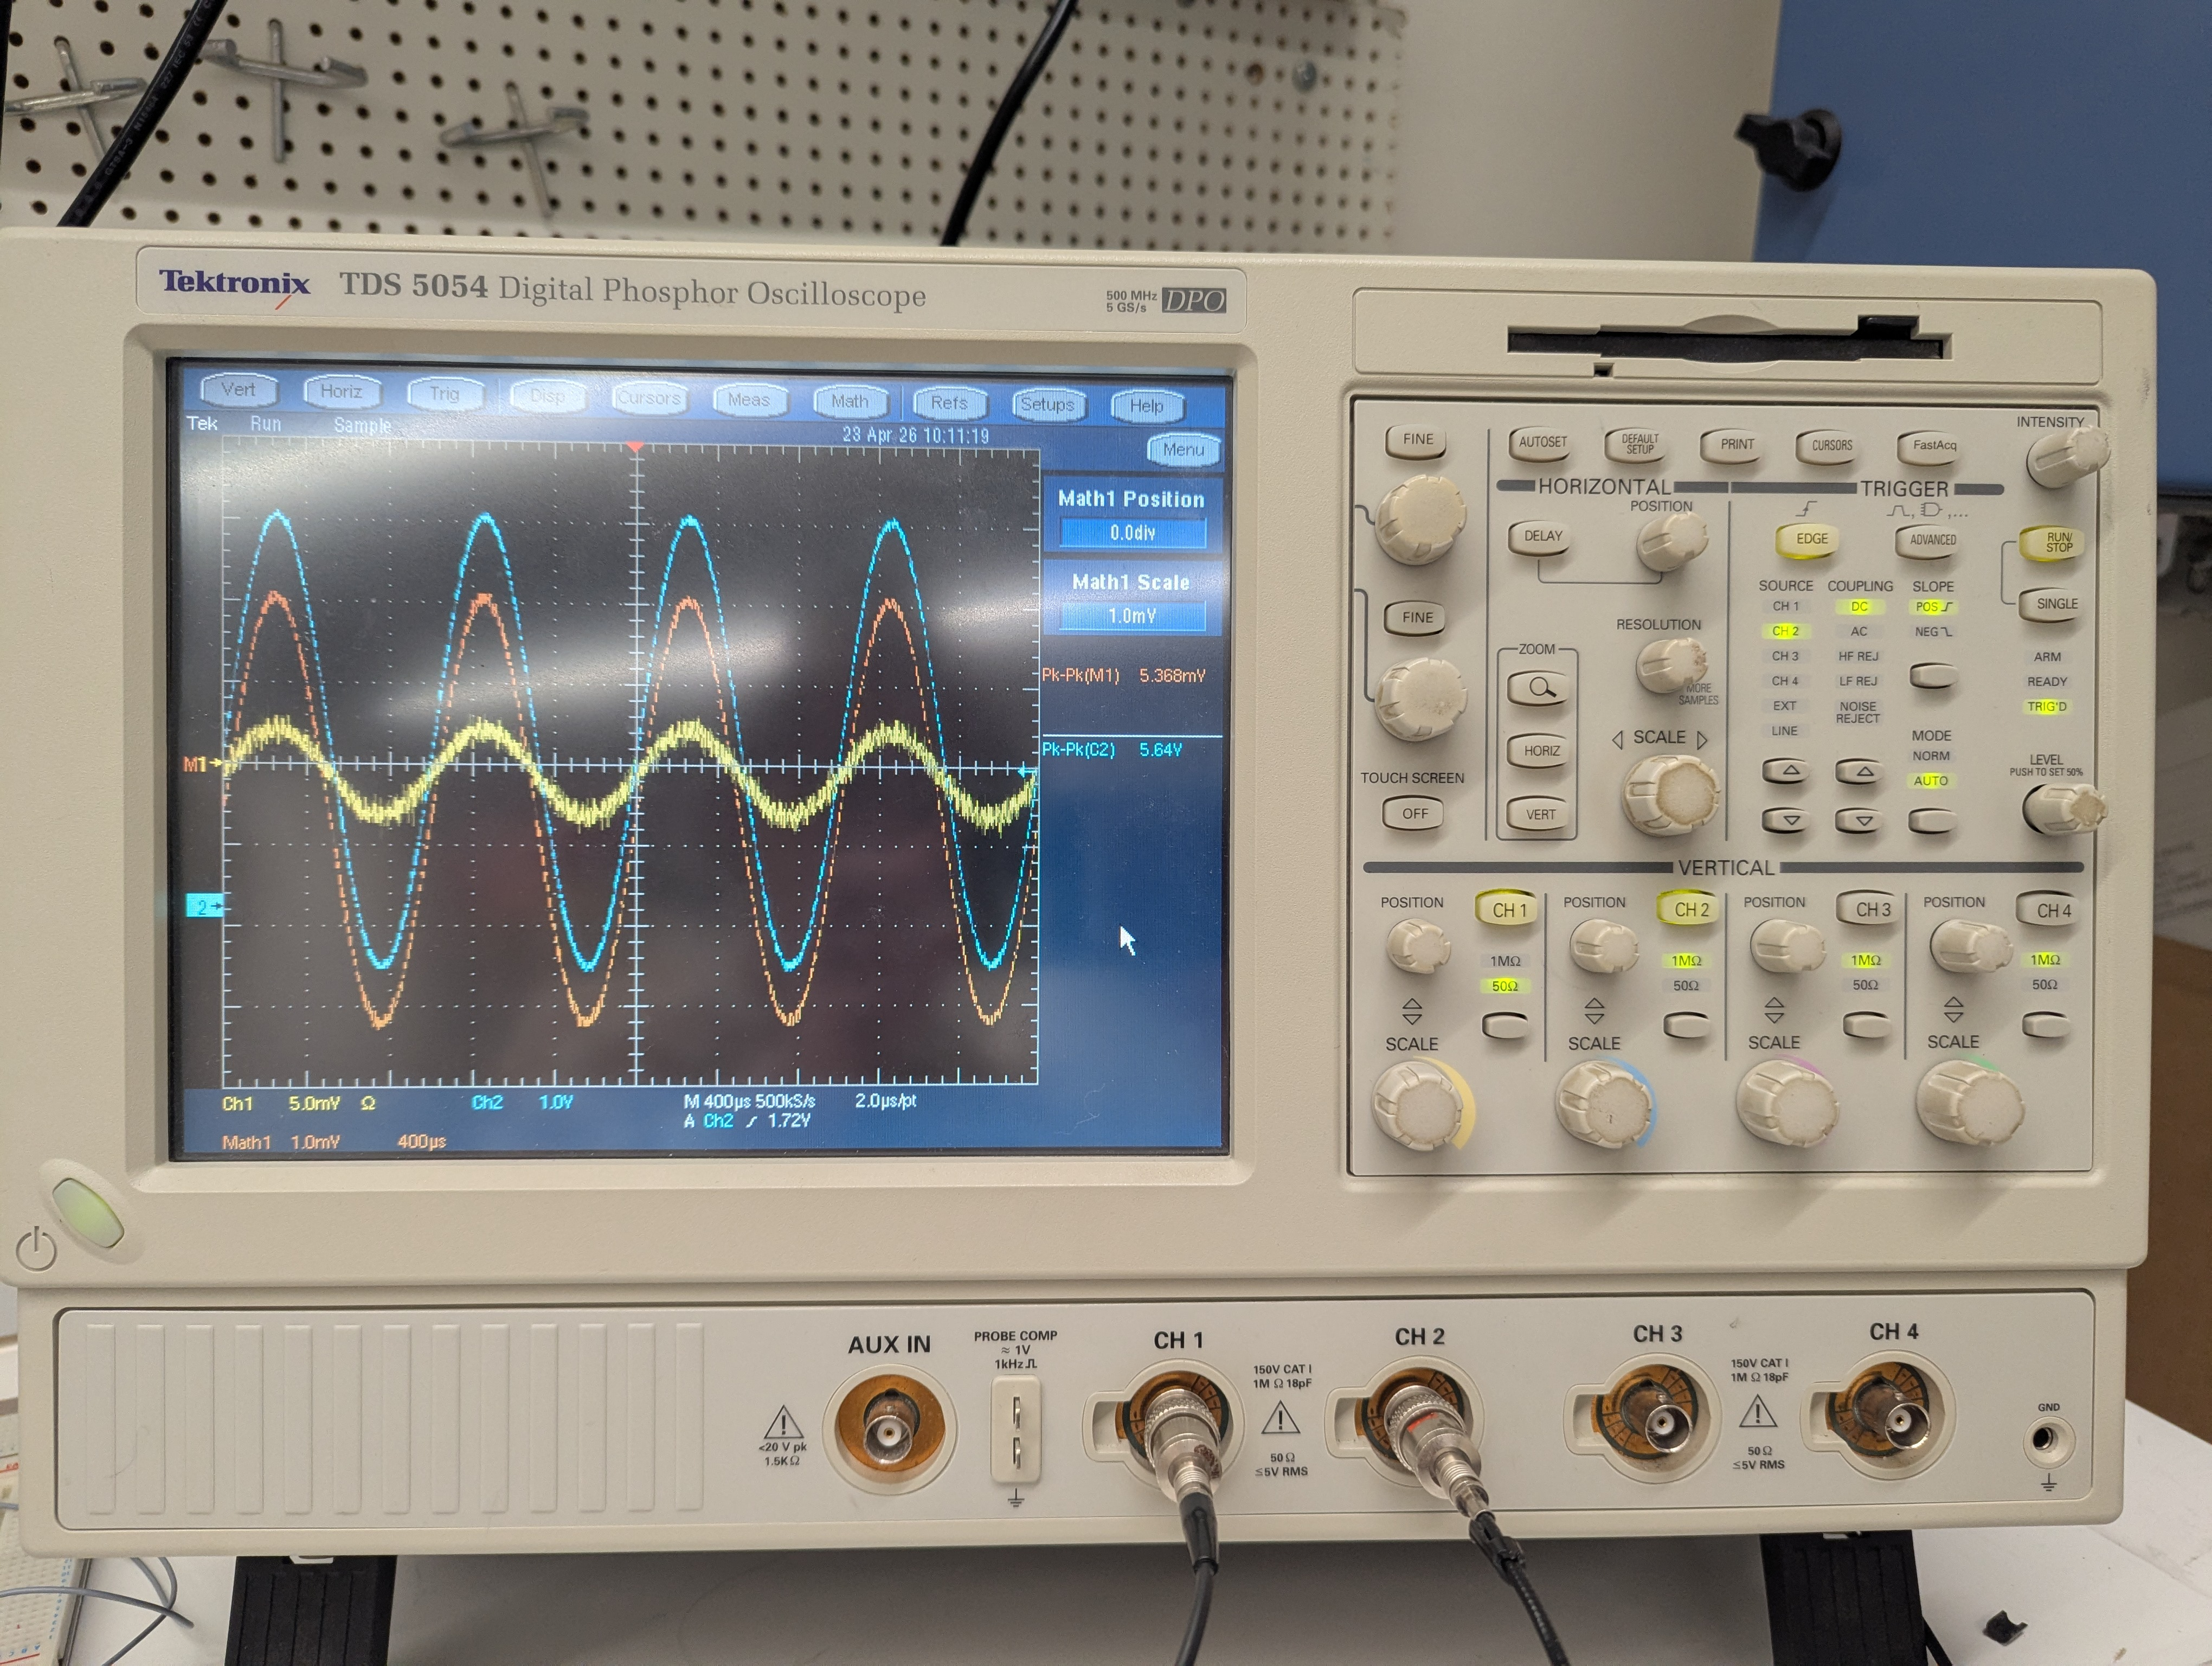
\includegraphics[width=\textwidth]{gain2.jpg}
  \end{minipage}
  \caption{Gain measurements of the operational amplifier circuit.
    The input to the circuit is on channel 1 (yellow), the output on channel 2 (blue)
    and \textit{Math1} (orange) shows the average of channel 1 over time.}
  \label{fig:gain-measurement}
\end{figure}

\begin{equation*}
  G = \frac{\overline{U}_\text{out,\,pp}}{\overline{U}_\text{in,\,pp}} = \frac{\SI{5.72}{\V} + \SI{5.64}{\V}}{\SI{5.404}{\mV} + \SI{5.368}{\mV} \approx 1058}
\end{equation*}



\clearpage
\printbibliography

\end{document}